\documentclass{article}
\usepackage{geometry, graphicx, float, subfigure, amsmath, bm, threeparttable, natbib, verbatim, indentfirst}
\usepackage[justification=centering]{caption}
\usepackage[marginal]{footmisc}
\geometry{a4paper,scale=0.8}
\setlength{\parindent}{2em}

\title{\bf{Financial Analysis of S\&P via Python}}
\author{Xueqing Tong}
\date{May 2019}

\begin{document}
    \begin{titlepage}
        \maketitle
        \setcounter{page}{0}
        \thispagestyle{empty}
    \end{titlepage}

    \renewcommand{\abstractname}{Introduction}
    \begin{abstract}
        From Physics 77, we have learnt to make use of python to process,analyze and display data. Since our group have interested in stocks market, we decide to apply Python to Financial analysis.

        Our object of study is stock price of the S\&P 500 Component Stocks. S\&P 500 Component Stocks comprises 505 common stocks issued by 500 large-cap companies and traded on American stock exchanges. 

        Our goals are as shown: First, we want to explore the correlation among the stock prices of different companies. Second, we want to give advice on whether to buy the stocks or not. Third, we want to predict the stocks prices accurately.
    \end{abstract}



    \section{Method}
    
        \subsection{Data Retrieving}
        With Python libraries as \verb!requests, BeautifulSoup, datetime! and \verb!pandas.datareader.data!, we easily get data on the S\&P 500 companies from the Yahoo Finance website and save them in csv. However, we met with a problem that we can't find stock price of Berkshire Hathaway (BRK.B). Later, we found out that Berkshire Hathaway was listed as BRK.B on Wikipedia from which we get all the tickers, but in Yahoo, we need to search Berkshire Hathaway as BRK-B.

        Then to make these data easier to handle with, we compile them into \verb!pandas.DataFrame!.

        \subsection{Pearson Correlation Calculation}
        We calculate and visualize Pearson correlations between each of the S\&P 500 stocks, further categorize companies by sectors, and then find and visualize the correlation within sectors. 
        
        The Pearson correlation measures the degree of a linear association between two variables and we always denote the Pearson correlation by $r$. The Pearson correlation coefficient, $r$, is between +1 and -1. A value of 0 indicates that there is totally no linear association between the two variables. The value of a positive number represents a positive association between the two variables while the value of a negative number represents a negative association between the two variables.
        
        Here we use \verb!colormap! of \verb!matplotlib! to present the correlation table. The table's tickers of horizontal and vertical coordinates are the abbreviation of company names. The point located at $(X, Y)$ represents the Pearson correlation of stock prices between $X$ company and $Y$ company in a long term. The color of each point corresponds to the value of the Pearson correlation as colorbar shows. 
    
        \subsection{Price Prediction}
        To predict the stock price in the future, we apply machine learning. \verb!Tensorflow! is a popular machine learning framework that simplifies the process of acquiring data, training models and serving predictions.
        
        Here, we make use of \verb!Tensorflow! to create a very simple three-layer neural network. We feed the input data X and output data Y as training sample to train the model. Input data is a feature matrix $X_{749\times995}$ and output data is a label matrix $Y_{749\times199}$. Every row of $X$ is 5 days data of 199 companies $(5 \times 199 = 995)$, and there are 749 rows (749 days in total data). Every row of $Y$ is the 6th day data of all the companies, and there are 749 rows. After training the model, we feed new input data into the model to predict the future stock prices of 199 companies.             
        
        In addition, S\&P 500 includes 505 companies, but we can not get stock prices of all the companies in a certain period. So we only include 199 companies.
    
        \subsection{Moving Average Calculation}
        We further calculate simple and weighted moving averages of different timescales for each stock, and compare it to the graph of the raw value of the stock. Here we calculate SMA and EMA and graph it. The simple moving average (SMA) calculates an average of the last 100 days' prices. The exponential moving average (EMA) is a weighted average of the last 21 days' prices, where the weighting of each previous price decreases exponentially with time. So we can see EMA gives recent prices more weight than past prices.
        
        Then we calculate the first and second derivative of the simple moving average for each stock and graph it. Here, we just use the first and second derivative to determine when to buy and sell a stock. To test accuracy of our buy-hold-sell method, we write a function: \verb!accuracy test()!. The probability of predicting successfully is about 30\%.
    
    \section{Conclusion}
    First, from Figure \ref{fig1}, we can see clearly that the correlation table is mostly green. It is reasonable that when the economy grows up, most companies perform well and thus the stock prices of companies go up altogether. On the contrary, when the economy is in recession, most companies perform bad and thus the stock prices of companies go down altogether.
   
    \begin{figure}[H]
        \centering
        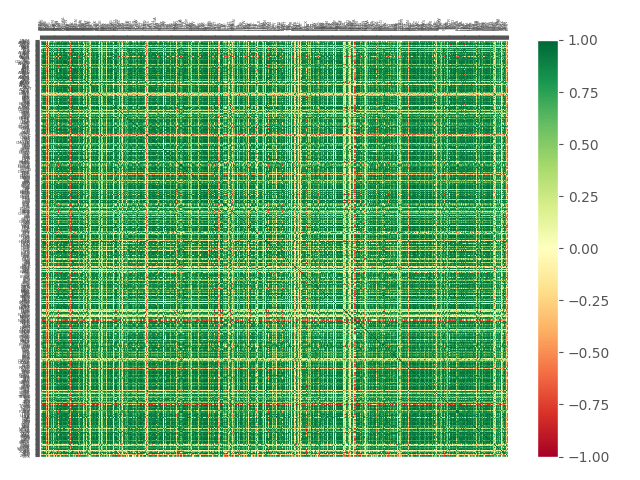
\includegraphics[width = 0.5\textwidth]{./1.png}
        \caption{S\&P 500 Correlation Table}
        \label{fig1}
    \end{figure}

    Second, we can see that correlation table can tell how companies with the same sectors compete and cooperate with each other. Take industrial sector for instance, we can see the stock price of General Electric (GE) has a negative correlation with almost all other companies' stock price. It can be explained by that electric power supply is relatively stable. When the economy grows up, the supply goes down compared with the growth of others and when the economy declines, the supply goes up compared with others. So GE has negative relationship with most other companies.

    \begin{figure}[H]
        \begin{minipage}[t]{0.45\textwidth}
            \centering
            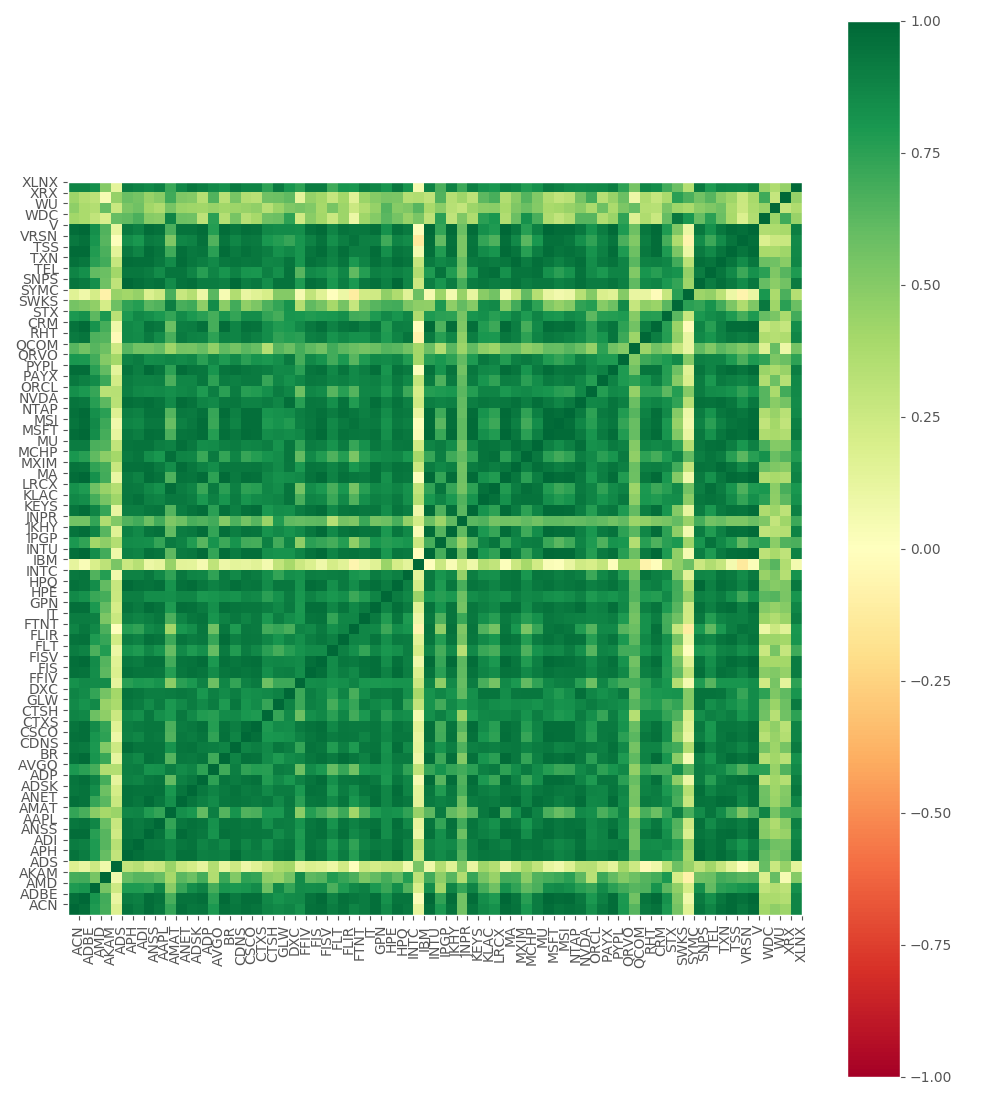
\includegraphics[width = 0.95\linewidth]{./3.png}
            \caption{Information Technology}
            \label{fig2}
        \end{minipage}
        \begin{minipage}[t]{0.45\textwidth}
            \centering
            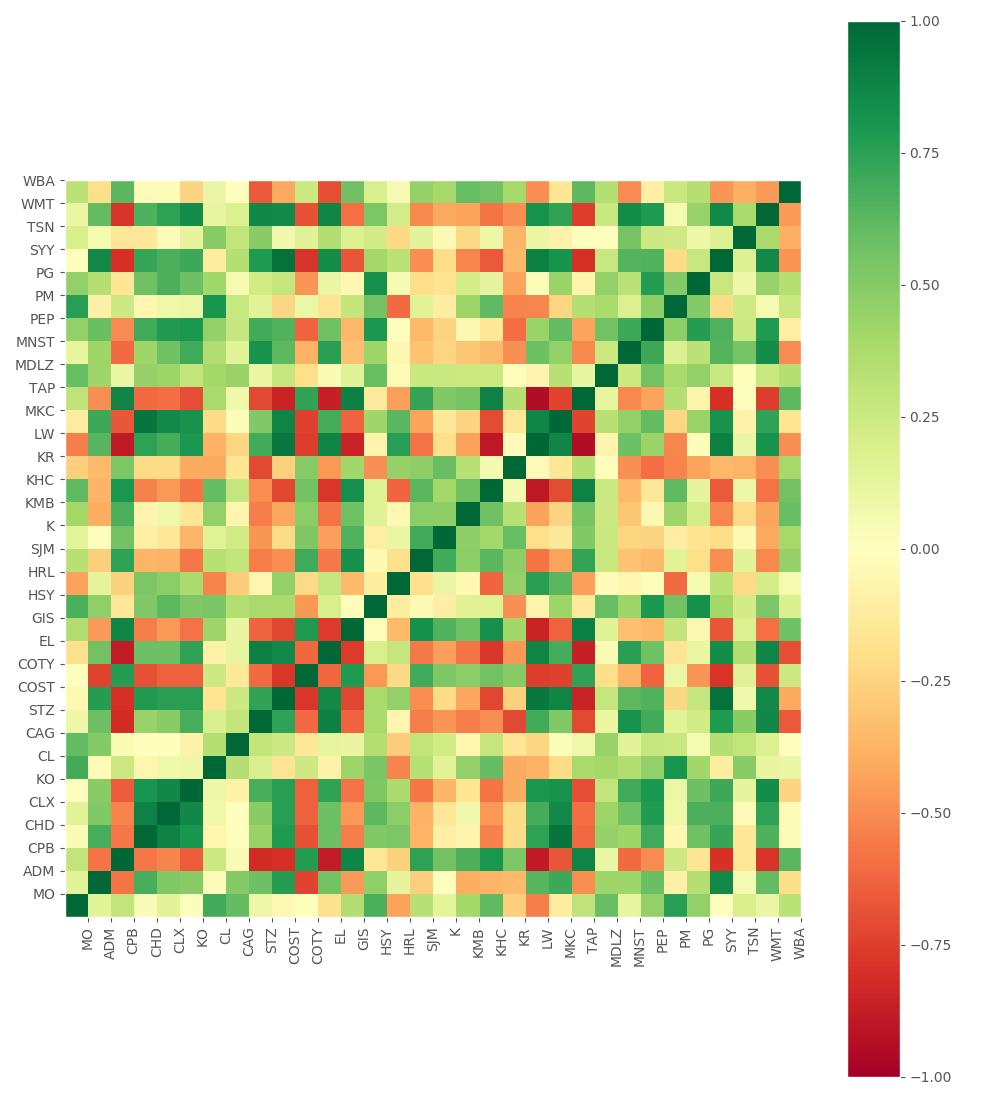
\includegraphics[width = 0.95\linewidth]{./2.png}
            \caption{Consumer Staple}
            \label{fig3}
        \end{minipage}
    \end{figure}

    We can also see that correlation table can tell how different sectors perform differently from others. In Figure \ref{fig2}, compared with other sectors, Information Technology is especially "green". Information Technology has grown up in recent decades. The whole sector perform well, so they are positively related. In Figure \ref{fig3}, it is not the case as for Consumer Staple. From the color of table, we can see that there is more competition among companies since the whole market for Consumer Staple is relatively stable.

    \begin{figure}[H]
        \centering
        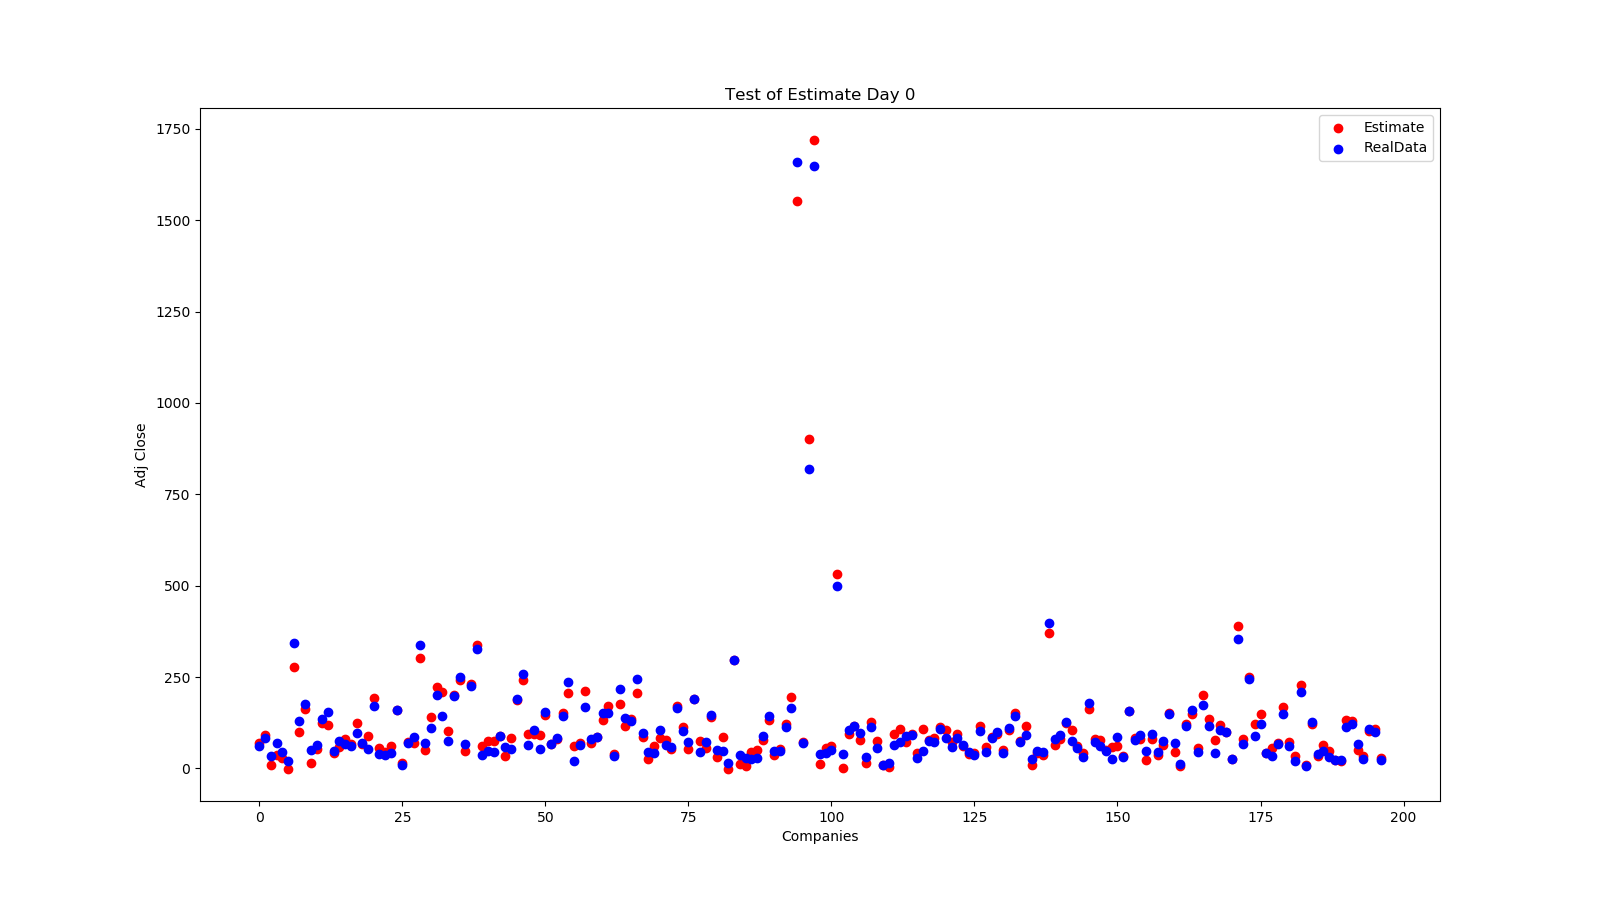
\includegraphics[width = 0.9\textwidth]{./4.png}
        \caption{Prediction and Real Data Comparison}
        \label{fig4}
    \end{figure}

    Third, in Figure \ref{fig4} we can see the prediction made by \verb!Tensorflow! framework is not that good. It is easy to understand that stock price is also influenced by other important factors like market sentiment and companies' financial status. So the knowledge that we feed the neural network is not enough. Meanwhile, the very simple three-layer neural network that we create may be too simple. So there is still room for further improvement.

\end{document}
